\documentclass[../main.tex]{subfiles}

\graphicspath{{../images/}}

\begin{document}
\pagestyle{fancy}

\lhead{Lecture 18: 10/31/24}
\chead{Chapter 8.1-8.2}
\rhead{PHYS 463}

\section{Equilibrium between Phases}
vapor $\rightleftharpoons$ water $\rightleftharpoons$ ice

\subsection{Isolated System}
\paragraph{General Aspects}:
\begin{itemize}
    \item For an isolated system, at equilibrium, the entropy is maximized
    \item For multiple systems, we must consider the entire system's entropy as a maximized quantity.
\end{itemize}

\paragraph{Case 1:} Isolated System
\begin{align*}
    Q &= \Delta \bar E + W \\
    W &= 0, Q = 0, \Delta \bar E = 0
\end{align*}
For some fluctuation:
\begin{align*}
    P(y) \propto \Omega (y) = e^{S(y)/k}, \quad
    \frac{P(y)}{P(\tilde y)} = \frac{e^{S(y)/k}}{e^{S(\tilde y)/k}} = e^{\Delta S/k}
\end{align*}
where the relative prob is exponentially suppressed.

\subsection{System in Contact with a Reservoir}
\paragraph{Case 2:} System is in contact with a reservoir at $T$
\begin{align*}
    A' + A = A^{(0)}
\end{align*}
where $S^{(0)}$ is maximized
\begin{align*}
    \Delta S^{(0)} \geq 0 = \Delta S + \Delta S'
\end{align*}
Heat transfer from the heat reservoir $A'$ (which doesn't change in Tempertature) to the system $A$ is
\begin{align*}
    \Delta S' = -\frac{Q}{T_0}
\end{align*}
In additiion, there is no work done on the system i.e. $Q = \Delta \bar E$ so
\begin{align*}
    \Delta S^{(0)} = \Delta S - \frac{Q}{T_0} = \frac{T_0 \Delta S - \Delta \bar E}{T_0} = \frac{\Delta (T_0 S - \bar E)}{T_0} 
    = \frac{-F_0}{T_0}
\end{align*}
where
\begin{align*}
    F_0 = T_0 S - \bar E
\end{align*}
is the Helmholtz free energy of system $A$ as it has the same temperature of the reservoir. 
Furthermore,
\begin{align*}
    \Delta F_0 \leq 0
\end{align*}
So the equilibrium condition requires a minimized free energy!

\newpage
\lhead{Lecture 19: 11/5/24}
\chead{Chapter 8.3-8.4}

\subsection{System in Contact with Reservoir at Constant Temperature and Pressure}
\paragraph{Review}:
\begin{itemize}
    \item Case I: Isolated system:
    \begin{align*}
        S \textrm{maximum}: \Delta S \geq 0
    \end{align*}
    \item Case II: Systme is contact with reservoir: Minimized `Helmholtz' free energy at constant temperature
    \begin{align*}
        \bar F_0 = \bar E - T_0 S
    \end{align*}
    \item Case III: System in contact with reservoir at constant $T_0, P_0$
    \begin{align*}
        A^{(0)} = A + A' \\
        \implies \Delta S^{(0)} = \Delta S + \Delta ' \geq 0 \quad \Delta S' = -\frac{Q}{T_0}
    \end{align*}
    so the entropy of the system and reservoir must increase by
    \begin{align*}
        \Delta S^{(0)} = \Delta S - \frac{Q}{T_0} = \frac{1}{T_0} (T_0 \Delta S - Q)
    \end{align*}
    where
    \begin{align*}
        Q = \Delta \bar E + P_0 \Delta V
    \end{align*}
    And doing some math movement, we find 
    \begin{align*}
        &= \frac{1}{T_0} (T_0 \Delta S - (\Delta \bar E + P_0 \Delta V)) \\
        &= \frac{1}{T_0} (\Delta (T_0 S - (\bar E + P_0 V)))
    \end{align*}
    or
    \begin{align*}
        \Delta S^{(0)} = -\frac{1}{T_0} \Delta G_0 \geq 0 \implies G_0 \leq 0
    \end{align*}
    So the equilibrium contision is: ``Gibbs free energy is minimized''
\end{itemize}

\subsection{Stability of homogeneous substance}
For the homogeneous substance, the Gibbs free energy is at a minimum
\begin{align*}
    G_0 \equiv \bar E - T_0 S + P_0 V
\end{align*}
and assume at equilibrium, subsystem $A$ is at $\tilde T, \tilde P$.

Fix $V$ and change $T$:
\begin{align*}
    \qt(\pdv{G_0}{T})_V = 0 \qqtext{for} T = \tilde T
\end{align*}
or using the definition
\begin{align*}
    \qt(\pdv{G_0}{T})_V = \qt(\pdv{\bar E}{T})_V - T_0 \qt(\pdv{S}{T})_V = 0
\end{align*}
where $T dS = d\bar E$ so
\begin{align*}
    \qt(\pdv{S}{T})_V = \qt(\pdv{\bar E}{T})_V \frac{1}{T}
\end{align*}
Therefore
\begin{align*}
    \pdv{G_0}{T}_V = \qt(\pdv{\bar E}{T})_V \qt(1 - \frac{T_0}{T}) = 0
\end{align*}
or $\tilde T = T$ at equilibrium.

Looking at the second derivative
\begin{align*}
    \qt(\pdv[2]{G_0}{T})_V &= \qt(\pdv[2]{\bar E}{T})_V \qt(1 - \frac{T_0}{T}) + \qt(\pdv{\bar E }{T})_V \qt(\frac{T_0}{T^2}) = 0 \\
    &= \qt(\pdv{\bar E }{T})_V \qt(\frac{T_0}{T^2}) = 0
\end{align*}
where
\begin{align*}
    C_V = \qt(\pdv{\bar E}{T})_V \geq 0
\end{align*}

\paragraph{Worksheet}
\begin{itemize}
    \item [1.]
    \begin{align*}
        \qt(\pdv{G_0}{V})_T = \qt(\pdv{\bar E}{V})_T - T_0 \qt(\pdv{S}{V})_T + P_0 = 0
    \end{align*}
    and from the fundamental relation
    \begin{align*}
        T \pdv{S}{V} = \pdv{\bar E}{V} + \bar P
    \end{align*}
    we have (using $T = T_0$)
    \begin{align*}
        \qt(\pdv{G_0}{V})_T &= \pdv{\bar E}{V} - \frac{T_0}{T} \qt(\pdv{E}{V} + \bar P) + P_0 = 0 \\
        &= P_0 - \bar P = 0 \implies P_0 = \bar P
    \end{align*}
    \item [2.] For the stability condition; the second derivative of $G_0$ must be positive
    \begin{align*}
        \qt(\pdv[2]{G_0}{V})_T = \qt(\pdv[2]{\bar E}{V})_T - T_0 \qt(\pdv[2]{S}{V})_T + 0 \geq 0
    \end{align*}
    and again
    \begin{align*}
        T \pdv[2]{S}{V} = \pdv[2]{\bar E}{V} + \pdv{\bar P}{V}
    \end{align*}
    so
    \begin{align*}
        \qt(\pdv[2]{G_0}{V})_T = -\qt(\pdv{\bar P}{V}) \geq 0 \implies \kappa = -\qt(\pdv{\bar P}{V}) \geq 0
    \end{align*}
    where $\kappa$ is the compressibility of the system.
\end{itemize}

\newpage
\lhead{Lecture 20: 11/7/24}
\chead{Chapter 8.5}
\subsubsection{Equilibrium between Phases}
Consider a single component system consisting of two phases 1, 2, e.g., liquid \& gas, liquid \& solid.

For certain equilibrium, phases can co-exist; the $G_0$ must still be a minimum
\begin{itemize}
    \item Assume:
    \begin{align*}
        n_1 &= \textrm{\# of moles in phase 1} \\
        n_2 &= \textrm{\# of moles in phase 2} \\
        g_1: &\textrm{Gibbs free energy per more of phase 1} \\
        g_2: &\textrm{Gibbs free energy per more of phase 2}
    \end{align*}
    \item At $T, P$
    \begin{align*}
        G &= n_1 g_1 + n_2 g_2 \quad n_1 + n_2 = n \\
        G &= (n - n_2) g_1 + n_2 g_2
    \end{align*}
\end{itemize}
So at equilibrium $G$ is a a minimum
\begin{align*}
    dG &= -g_1 dn_2 + g_2 dn_2 \\
    &= (g_2 - g_1) dn_2 = 0 \implies g_1(T,P) = g_2(T,P)
\end{align*}
or a phase equilibrium line on the $T-P$ diagram.

At a point $B$ on the line,
\begin{align*}
    g_1(T + dT, P + dP) = g_2(T + dT, P + dP)
\end{align*}
or
\begin{align*}
    dg_i = \qt(\pdv{g_i}{T})_P dT + \qt(\pdv{g_i}{P})_T dP 
\end{align*}
So using the fundamental relation (where the lower case is the per molar quantity)
\begin{align*}
    dg = d (\epsilon - Ts + Pv) = -s dT + v dP 
\end{align*}
And at the equilibrium point $B$
\begin{align*}
    dg_1 = dg_2 = \implies - s_1 dT + v_1 dP = - s_2 dT + v_2 dP
\end{align*}
or rewritten as
\begin{align*}
    (s_2 - s_1) dT = (v_2 - s_1) dP \implies \dv{P}{T} = \frac{\Delta s}{\Delta s}
\end{align*}
We can see that $dP/dT$ is the slope of the line on the $T-P$ diagram AKA the `Clausius-Clapeyron equation'.
Using the definition $\Delta S = Q / T$ or latent heat of transformation from phase 1 to phase 2, $L_{12} = T \Delta S$:
\begin{align*}
    \dv{P}{T} = \frac{Q}{T \Delta V} = \frac{L_{12}}{T \Delta V}
\end{align*}

\newpage
\paragraph{Simple Phase Transformation:} Solid $\to$ Liquid:
\begin{itemize}
    \item Entropy $\uparrow$ increases
    \item Absorb heat
\end{itemize}

% water_pt.png
\begin{figure}[ht]
    \centering
    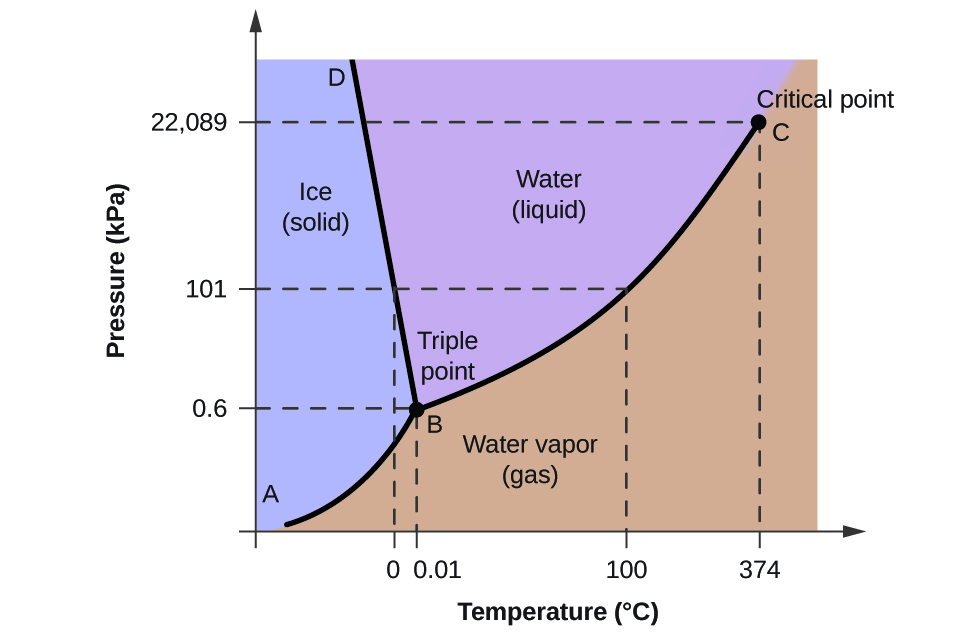
\includegraphics[width=0.8\textwidth]{water_pt.png}
    \caption{Phase diagram of water}
    \label{fig:water_pt}
\end{figure}

\paragraph{Worksheet}
\begin{itemize}
    \item For a phase diagram similar to water, as melt from Solid to Liquid,
    the pressure decrease, so the material expands.
    \item Using the CC equation
    \begin{align*}
        dP &= \frac{L_{12}}{T \Delta V}  dT \\
        \implies \Delta P &= \int L_{12} \frac{dT}{T \Delta V} = \frac{L_{12}}{\Delta V} \ln \frac{T_2}{T_1}
    \end{align*}
    As an ideal gas $pv = RT \implies v = RT / p$ so 
    \begin{align*}
        \dv{p}{T} = \frac{p l_{12}}{RT^2} \\
        \frac{1}{p} dp = \frac{l_{12}}{RT^2} dT
    \end{align*}
    integrating both sides
    \begin{align*}
        \ln p = -\frac{l_{12}}{RT} + C
    \end{align*}
    or
    \begin{align*}
        p = p_0 e^{-l_{12}/RT}
    \end{align*}
    So pressure increases very very rapidly with $T$.
\end{itemize}

\newpage
\chead{Chapter 8.7}
\subsection{Chemical Equilibrium}
E.g. 
\begin{align*}
    2H_2 + O_2 \rightleftharpoons 2H_2O
\end{align*}
``Chemical potential'', systems with several components:

Consider a system with $\bar E, V$, m different kinds of components (e.g. molecules),
and $N_i$ number of each type:
\begin{align*}
    S = S(E, V, N_1, N_2, \dots, N_m)
\end{align*}
The number $N_i$ can change due to chemical reactions.

For general infinitesimal process
\begin{align*}
    dS = \qt(\pdv{S}{E})_{V, N} dE + \qt(\pdv{S}{V})_{E, N} dV + \sum_i \qt(\pdv{S}{N_i})_{E, V, N_{j\neq i}} dN_i
\end{align*}
where
\begin{align*}
    \pdv{S}{E} = \frac{1}{T}, \pdv{S}{V} = \frac{P}{T}
\end{align*}
and a new quantity
\begin{align*}
    \mu_i = - T \qt(\pdv{S}{N_i})_{E, V, N_{j\neq i}}
\end{align*}
or the ``chemical potential'' per molecule of of the ith species.
So we can rewrite to
\begin{align*}
    dS = \frac{1}{T} dE + \frac{P}{T} dV - \sum_i^m \frac{\mu_i}{T} dN_i
\end{align*}

\paragraph{Other forms} We can also express $\mu_i$ in different forms by moving stuff around:
\begin{align*}
    dE = T dS - p dV + \sum_i \mu_i dN_i
\end{align*}
or
\begin{align*}
    \implies \mu_i = \qt(\pdv{E}{N_i})_{S, V, N_{j\neq i}}
\end{align*}
In terms of the Helmholtz free energy
\begin{align*}
    F = E - TS \implies dF = d(E - TS)
\end{align*}
or
\begin{align*}
    \implies \mu_i = \qt(\pdv{F}{N_i})_{T, V, N_{j\neq i}}
\end{align*}
And in terms of the Gibbs free energy
\begin{align*}
    d(E - TS + pV) = dG
\end{align*}
so 
\begin{align*}
    \mu_i = \qt(\pdv{G}{N_i})_{T, P, N_{j\neq i}}
\end{align*}

If there is only 1 species of a molecule then
\begin{align*}
    G = G(T,p, N) = N g' (T,p) \implies \mu = g'(T,p)
\end{align*}

\end{document}